\documentclass[11pt,a4paper]{article}

% --- Packages ---
\usepackage[utf8]{inputenc}
\usepackage[T1]{fontenc}
\usepackage{lmodern}
\usepackage{amsmath,amssymb}
\usepackage{graphicx}
\usepackage{booktabs}
\usepackage[margin=1in]{geometry}
\usepackage{caption}
\usepackage{subcaption}
\usepackage{float}
\usepackage{microtype}
\usepackage{xcolor}
\usepackage[colorlinks=true,linkcolor=blue,citecolor=blue,urlcolor=blue]{hyperref}
\usepackage[numbers,sort&compress]{natbib}
\usepackage{url}
\usepackage{listings}
\usepackage{enumitem}
\usepackage{multirow}
\usepackage{siunitx}

% --- Figure path ---
\graphicspath{{../outputs/}}

% --- Caption formatting ---
\captionsetup[figure]{font=small,labelfont=bf,skip=6pt}
\captionsetup[table]{font=small,labelfont=bf,skip=6pt}

% --- Title ---
\title{
    \vspace{-1.5cm}
    \textbf{Energy-Aware Flexible Job-Shop Scheduling via a\\ Memetic NSGA-II}
    \vspace{0.5cm}
}
\author{
    Adeleke Olorunnisola Oyeyemi
}
\date{August 2026}

\begin{document}

\maketitle

\begin{abstract}
\noindent
This document describes the design, implementation, and results of a bi-objective optimisation
mini project that schedules the Flexible Job-Shop Scheduling Problem (FJSP) to jointly minimise
\textit{makespan} and \textit{energy cost}, where energy cost is computed from a real, time-varying
electricity price series rather than an assumed flat rate. The scheduler is a \emph{memetic
NSGA-II}: the multi-objective genetic algorithm NSGA-II \citep{deb2002fast}, hybridised with a
greedy local-search refinement step, and solving real Brandimarte \citeyearpar{brandimarte1993routing}
FJSP benchmark instances against real ENTSO-E day-ahead electricity prices (Belgium, February 2022).
The project is methodologically inspired by \citet{burmeister2024memetic}, who introduce and validate
a memetic NSGA-II for FJSP under real-time energy tariffs. This document covers the motivation,
problem formulation, algorithm design, data sources, implementation, and results, and closes with an
explicit comparison of what is simplified relative to the source paper. Source code and full results
are hosted at \url{https://github.com/Olorunnisola01/energy-aware-fjsp-nsga2}.
\end{abstract}

\tableofcontents
\newpage

% =====================================================================
\section{Introduction and Motivation}
\label{sec:introduction}
% =====================================================================

Electricity grids are incorporating increasing shares of intermittent renewable generation (wind,
solar), which introduces volatility into energy supply and, consequently, into energy prices
\citep{abujarad2017recent,gandhi2016review}. Under real-time pricing (RTP) tariffs, the cost of
electricity can change at hourly (or finer) intervals depending on current market conditions. This
creates an opportunity, and an incentive, for energy-flexible manufacturers to practice \emph{demand
response}: shifting production toward hours when energy is cheap, without any new capital investment
\citep{detorre2022exploiting}.

Job-shop scheduling problems are a natural setting for this idea. In the \emph{Flexible Job-Shop
Scheduling Problem} (FJSP), each job consists of a sequence of operations, and each operation may be
processed on any machine from a compatible subset, as opposed to the classical job-shop problem,
where each operation is tied to exactly one machine. This flexibility gives a scheduler room to choose
\textit{when} and \textit{on which machine} to run an operation, which is exactly the freedom needed
to react to a time-varying energy price signal.

Minimising energy cost in isolation is not useful: a scheduler that always waits for the cheapest
possible price window will produce arbitrarily long schedules. The problem is therefore inherently
\emph{bi-objective}, simultaneously minimising makespan (total completion time) and energy cost, and
the interesting output is not a single ``best'' schedule but a \emph{Pareto front} of trade-offs
between the two, from which a decision-maker can pick according to their own priorities.

This project implements exactly that: a memetic NSGA-II that approximates the makespan/energy-cost
Pareto front for FJSP instances under a real RTP electricity price signal.

% =====================================================================
\section{Related Work}
\label{sec:related-work}
% =====================================================================

\subsection{Energy-Cost-Aware Scheduling}
\label{subsec:energy-cost-aware}

The literature on energy-cost-aware scheduling is organised around three tariff structures
\citep{burmeister2024memetic}:

\begin{enumerate}[label=\arabic*.]
    \item \textbf{Fixed rate}: a constant price regardless of time of consumption
    (e.g.\ \citet{carlucci2021job,kemmo2015job}).
    \item \textbf{Time-of-use (TOU) rate}: the day is divided into a small number of coarse-grained
    periods (e.g.\ off-peak / mid-peak / on-peak), each with its own price
    (e.g.\ \citet{zhang2014energy,biel2018flow}).
    \item \textbf{Real-time pricing (RTP)}: the price is based on the current market value of energy
    and can change at hourly or finer intervals (e.g.\ \citet{gong2015energy,shrouf2014optimizing}).
\end{enumerate}

\citet{burmeister2024memetic} identify a gap in this literature: prior RTP-based work is largely
restricted to single-machine or flow-shop settings and single-objective (energy-cost-only)
formulations, or neglects makespan optimisation entirely. Their paper closes this gap with a
\emph{multi-objective}, RTP-aware FJSP formulation solved by a memetic NSGA-II, validated
computationally against an exact Gurobi solver on the Brandimarte \citeyearpar{brandimarte1993routing}
benchmark suite.

\subsection{NSGA-II and Memetic Algorithms}
\label{subsec:nsga2-memetic}

NSGA-II \citep{deb2002fast} is a widely used multi-objective evolutionary algorithm. It maintains a
population of candidate solutions, ranks them into non-dominated fronts, and uses a crowding-distance
measure to preserve diversity along each front, producing, generation over generation, an
approximation of the true Pareto front rather than a single solution.

A \emph{memetic algorithm} \citep{moscato2003gentle} augments a population-based metaheuristic with a
local-search refinement step applied to individuals (typically offspring), combining the global
exploration of an evolutionary algorithm with the fast local exploitation of a hill-climbing search.
\citet{burmeister2024memetic} apply this idea to NSGA-II for FJSP; this project follows the same
combination.

\subsection{Benchmark Instances}
\label{subsec:benchmark}

\citet{brandimarte1993routing} introduced a set of fifteen FJSP benchmark instances (mk01--mk15),
commonly used in the FJSP literature (and by \citet{burmeister2024memetic}) as a standard testbed.
This project uses ten of these instances (mk01--mk10), parsed from the standard Hurink
\texttt{.fjs} text format.

% =====================================================================
\section{Problem Formulation}
\label{sec:problem-formulation}
% =====================================================================

\subsection{Inputs}
\label{subsec:inputs}

\begin{itemize}
    \item A set of jobs $\mathcal{J} = \{1, \ldots, n\}$, each consisting of an ordered sequence of
    operations that must be processed in sequence.
    \item A set of machines $\mathcal{M} = \{1, \ldots, m\}$.
    \item For each operation, a subset of machines that can process it, and a processing time for
    each such machine (processing time may differ by machine).
    \item A real-valued electricity price series $p(t)$ (EUR/kWh), giving the price of energy at
    every minute $t$ of the planning horizon.
\end{itemize}

\subsection{Decision Variables}
\label{subsec:decision-variables}

For every operation:
\begin{enumerate}[label=\arabic*.]
    \item \textbf{Machine assignment}: which eligible machine processes the operation.
    \item \textbf{Sequencing position}: the relative order in which operations are dispatched,
    subject to (a) machine availability (a machine processes one operation at a time) and (b) job
    precedence (an operation cannot start before the previous operation of the same job finishes).
\end{enumerate}

\subsection{Objectives}
\label{subsec:objectives}

\begin{align}
    \min f_1 &= \text{makespan} = \max_{i} \left( \text{completion time of operation } i \right) \\
    \min f_2 &= \text{energy cost} = \sum_{i} \int_{\text{start}_i}^{\text{end}_i} p(t) \, dt
\end{align}

where the integral for each operation $i$ is evaluated exactly by summing the per-minute price over
that operation's start/end window. No feasible solution can simultaneously minimise both objectives (a
faster schedule generally cannot always wait for the cheapest price window), so the output is a
Pareto-optimal set of trade-offs rather than one optimum.

% =====================================================================
\section{Methodology}
\label{sec:methodology}
% =====================================================================

\subsection{Solution Encoding}
\label{subsec:solution-encoding}

A candidate solution is encoded as a vector of length $2 \times n_{\text{ops}}$:
\begin{itemize}
    \item The first half assigns, for each operation, an integer machine-choice index, taken modulo
    the number of machines eligible for that specific operation (so any integer is a valid, decodable
    gene, which avoids infeasible machine assignments by construction).
    \item The second half assigns each operation a sort key; operations are dispatched in ascending
    order of this key, subject to machine and job-precedence availability (a standard
    permutation-based scheduling decoder).
\end{itemize}

\subsection{Memetic NSGA-II}
\label{subsec:memetic-nsga2}

The algorithm is standard NSGA-II (non-dominated sorting, crowding distance, tournament selection,
simulated-binary crossover and polynomial mutation for integer variables, via the \texttt{pymoo}
library) with one addition: after each generation produces its offspring, every offspring is refined
by a \emph{greedy local search} before being merged back into the population.

The local search alternates between two neighbourhood moves until neither improves the current
solution:
\begin{enumerate}[label=\arabic*.]
    \item \textbf{Machine re-assignment}: for each operation, try the next eligible machine; keep
    the move if it Pareto-dominates the current solution.
    \item \textbf{Sequencing swap}: for each pair of operations, try swapping their sequencing keys;
    keep the move if it Pareto-dominates the current solution.
\end{enumerate}

This hybridises NSGA-II's global, population-level search with fast, solution-level exploitation,
which is the core idea of a memetic algorithm \citep{moscato2003gentle} and the central
methodological device in \citet{burmeister2024memetic}.

\subsection{Duplicate Removal}
\label{subsec:duplicate-removal}

NSGA-II's population can end a run containing multiple genotypes that decode to the same schedule
(and therefore the same objective values). The final reported Pareto front is deduplicated
(\texttt{numpy.unique} on objective values) so it reads as a clean, strictly non-dominated set rather
than a front inflated with repeated points.

% =====================================================================
\section{Data}
\label{sec:data}
% =====================================================================

\subsection{Benchmark Instances}
\label{subsec:data-benchmark}

Ten Brandimarte \citeyearpar{brandimarte1993routing} FJSP benchmark instances are used, mk01--mk10,
parsed from the standard Hurink \texttt{.fjs} text format (machine indices 0-based; each job line
lists its operation count, then for each operation its number of eligible machines followed by
machine/time pairs). Instance files were sourced from the \texttt{SchedulingLab/fjsp-instances}
public repository \citep{schedulinglab_fjsp} and independently validated (every token in every file
was checked to parse into a complete, internally consistent operation list with no leftover or
missing tokens) before use.

\begin{table}[htbp]
    \centering
    \caption{Brandimarte (1993) FJSP benchmark instances used in this project.}
    \label{tab:benchmark-instances}
    \begin{tabular}{lcc}
        \toprule
        \textbf{Instance} & \textbf{Jobs} & \textbf{Machines} \\
        \midrule
        mk01 & 10 & 6 \\
        mk02 & 10 & 6 \\
        mk03 & 15 & 8 \\
        mk04 & 15 & 8 \\
        mk05 & 15 & 4 \\
        mk06 & 10 & 15 \\
        mk07 & 20 & 5 \\
        mk08 & 20 & 10 \\
        mk09 & 20 & 10 \\
        mk10 & 20 & 15 \\
        \bottomrule
    \end{tabular}
\end{table}

The results reported in this document use \texttt{mk01} (10 jobs, 6 machines, 55 operations).

\subsection{Electricity Price Data}
\label{subsec:data-price}

Real day-ahead electricity prices for the Belgian bidding zone, February 2022, were sourced from the
ENTSO-E Transparency Platform \citep{entsoe_transparency}. The raw export (EUR/MWh, timestamps like
``Feb 1, 2022 12:00 AM'') is preprocessed by \texttt{parsing\_data.py} into a clean
\texttt{(timestamp, price\_eur\_per\_kWh)} series, which is then resampled to per-minute resolution
at run time so that energy cost can be integrated exactly over each operation's start/end window
rather than approximated at hourly granularity.

% =====================================================================
\section{Implementation}
\label{sec:implementation}
% =====================================================================

The project is implemented in Python~3, using:
\begin{itemize}
    \item \texttt{pymoo} for the NSGA-II algorithm framework;
    \item \texttt{numpy}/\texttt{pandas} for numerical computation and price-series handling;
    \item \texttt{matplotlib} for all figures.
\end{itemize}

\begin{table}[htbp]
    \centering
    \caption{Key files in the project repository.}
    \label{tab:key-files}
    \begin{tabular}{lp{0.65\textwidth}}
        \toprule
        \textbf{File} & \textbf{Purpose} \\
        \midrule
        \texttt{nsga2\_fjsp\_energy.py} & Problem definition, memetic NSGA-II, plotting, CLI \\
        \texttt{parse\_fjs\_instance} (in the same file) & Hurink \texttt{.fjs} benchmark parser \\
        \texttt{parsing\_data.py} & One-off preprocessing of the raw ENTSO-E export \\
        \texttt{benchmarks/brandimarte/mk01.txt}--\texttt{mk10.txt} & Benchmark instance files \\
        \texttt{belgium\_prices\_feb2022.csv} & Cleaned electricity price series \\
        \bottomrule
    \end{tabular}
\end{table}

Both the benchmark instance choice and the NSGA-II run are fully specified by command-line arguments
and a random seed, so a given configuration reproduces the same Pareto front:

\begin{lstlisting}[language=bash,frame=single,numbers=none,basicstyle=\ttfamily\footnotesize]
python nsga2_fjsp_energy.py --instance mk01 --n-gen 800 --pop-size 20 --seed 42
\end{lstlisting}

A \texttt{--random} flag is retained for generating synthetic FJSP instances of arbitrary size,
independent of the benchmark suite.

% =====================================================================
\section{Experimental Setup}
\label{sec:experimental-setup}
% =====================================================================

\begin{table}[htbp]
    \centering
    \caption{Experimental configuration used for the reported results.}
    \label{tab:experimental-setup}
    \begin{tabular}{ll}
        \toprule
        \textbf{Parameter} & \textbf{Value} \\
        \midrule
        Benchmark instance & mk01 (10 jobs, 6 machines, 55 operations) \\
        Population size & 20 \\
        Generations & 800 \\
        Random seed & 42 \\
        Energy price series & Belgium, February 2022 (ENTSO-E), per-minute resolution \\
        \bottomrule
    \end{tabular}
\end{table}

% =====================================================================
\section{Results}
\label{sec:results}
% =====================================================================

\subsection{Convergence}
\label{subsec:convergence}

Both objectives improve steadily over generations and plateau well before the run ends, indicating
the population has converged. Figures~\ref{fig:convergence-makespan} and
\ref{fig:convergence-energy} show the best makespan and best energy cost, respectively, as a
function of the generation number.

\begin{figure}[htbp]
    \centering
    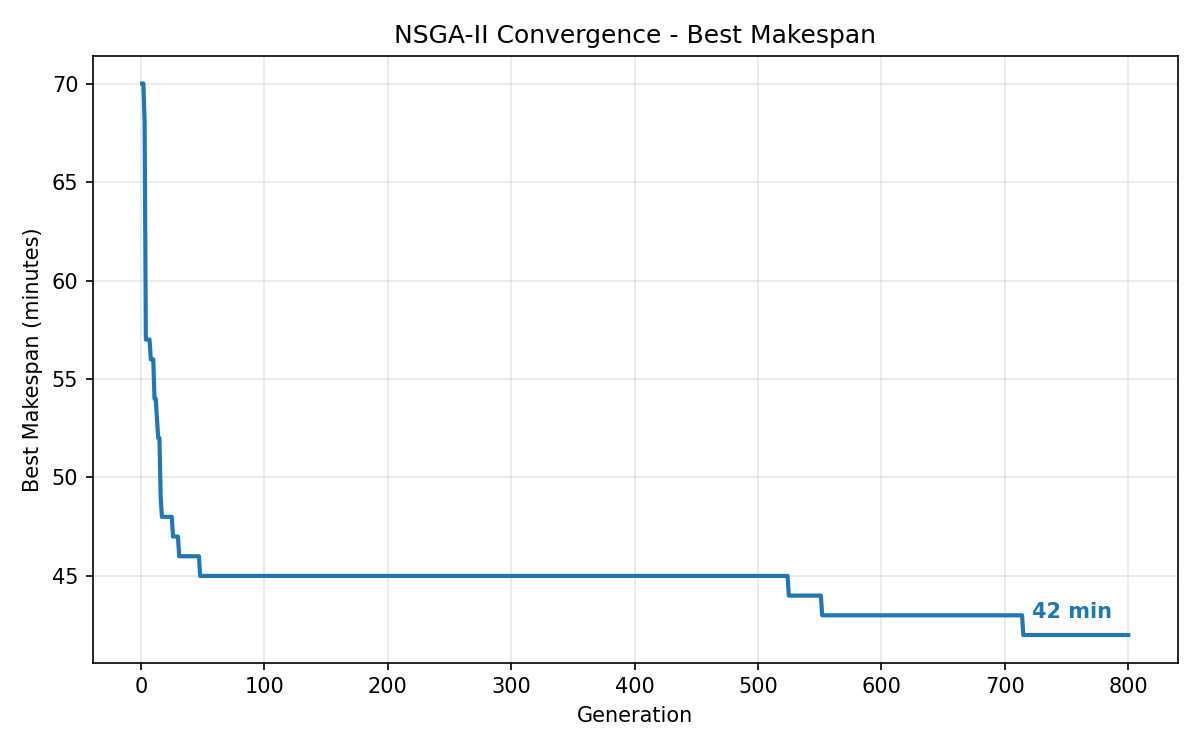
\includegraphics[width=0.75\textwidth]{convergence_makespan.png}
    \caption{Best makespan per generation.}
    \label{fig:convergence-makespan}
\end{figure}

\begin{figure}[htbp]
    \centering
    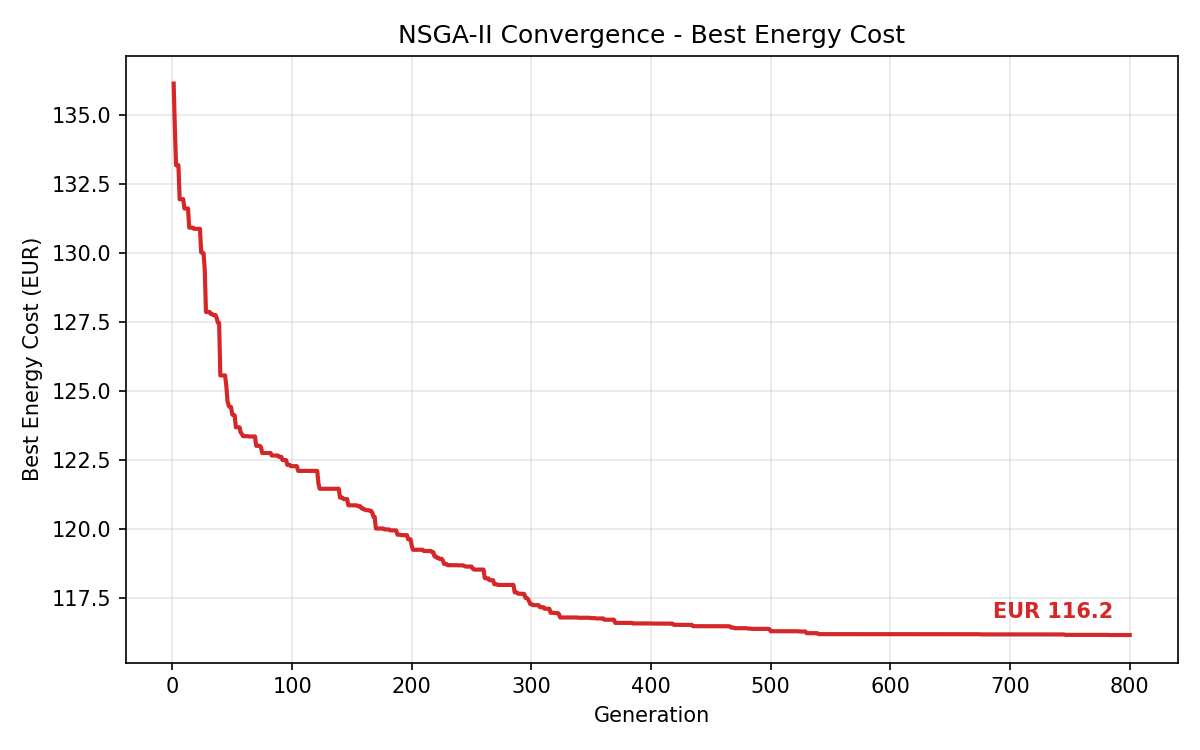
\includegraphics[width=0.75\textwidth]{convergence_energy.png}
    \caption{Best energy cost per generation.}
    \label{fig:convergence-energy}
\end{figure}

\subsection{Pareto Front}
\label{subsec:pareto-front}

The final, deduplicated Pareto front contains 15 non-dominated solutions, trading off a 42-minute
minimum-makespan schedule (higher energy cost) against an 88-minute schedule at the lowest energy
cost found. Figure~\ref{fig:pareto-front} plots the front, and Table~\ref{tab:pareto-front} lists
the full set of non-dominated objective values.

\begin{figure}[htbp]
    \centering
    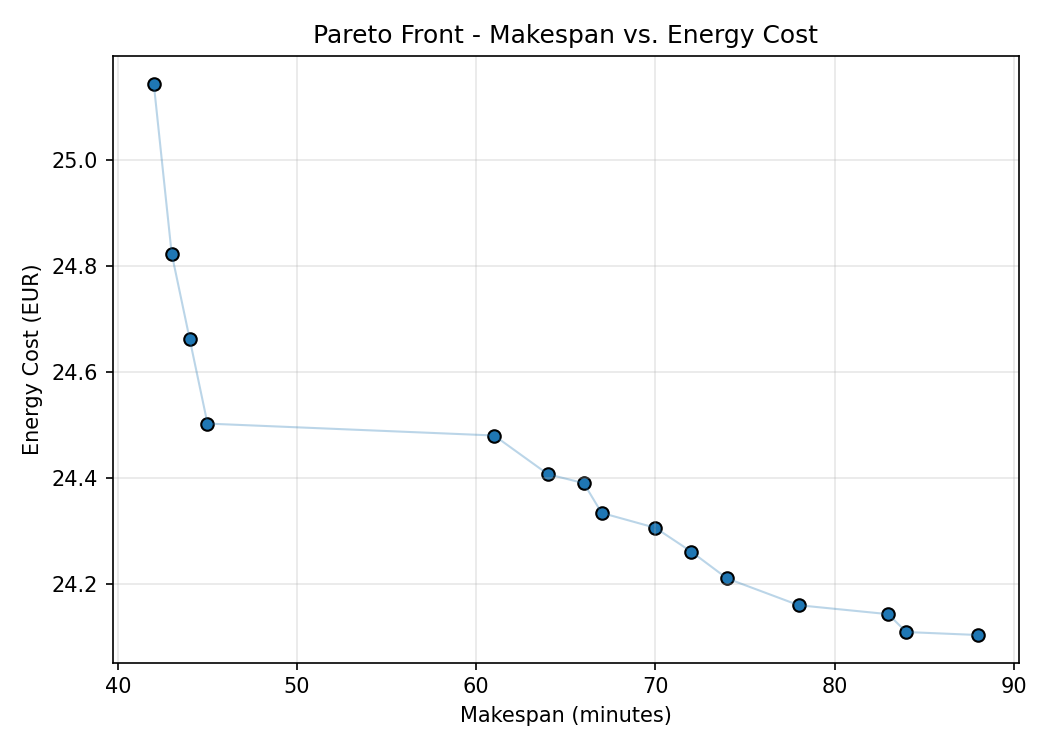
\includegraphics[width=0.7\textwidth]{pareto_front.png}
    \caption{Pareto front: makespan vs.\ energy cost.}
    \label{fig:pareto-front}
\end{figure}

\begin{table}[htbp]
    \centering
    \caption{Full Pareto front (makespan vs.\ energy cost), mk01, seed 42, 800 generations.}
    \label{tab:pareto-front}
    \begin{tabular}{cc}
        \toprule
        \textbf{Makespan (min)} & \textbf{Energy Cost (EUR)} \\
        \midrule
        42 & 25.14 \\
        43 & 24.82 \\
        44 & 24.66 \\
        45 & 24.50 \\
        61 & 24.48 \\
        64 & 24.41 \\
        66 & 24.39 \\
        67 & 24.33 \\
        70 & 24.31 \\
        72 & 24.26 \\
        74 & 24.21 \\
        78 & 24.16 \\
        83 & 24.14 \\
        84 & 24.11 \\
        88 & 24.10 \\
        \bottomrule
    \end{tabular}
\end{table}

\subsection{Schedule (Gantt Chart)}
\label{subsec:gantt}

The schedule below corresponds to the minimum-makespan solution on the Pareto front (42 minutes).
Each colour is a distinct job; bars are labelled with job/operation IDs where space allows.

\begin{figure}[htbp]
    \centering
    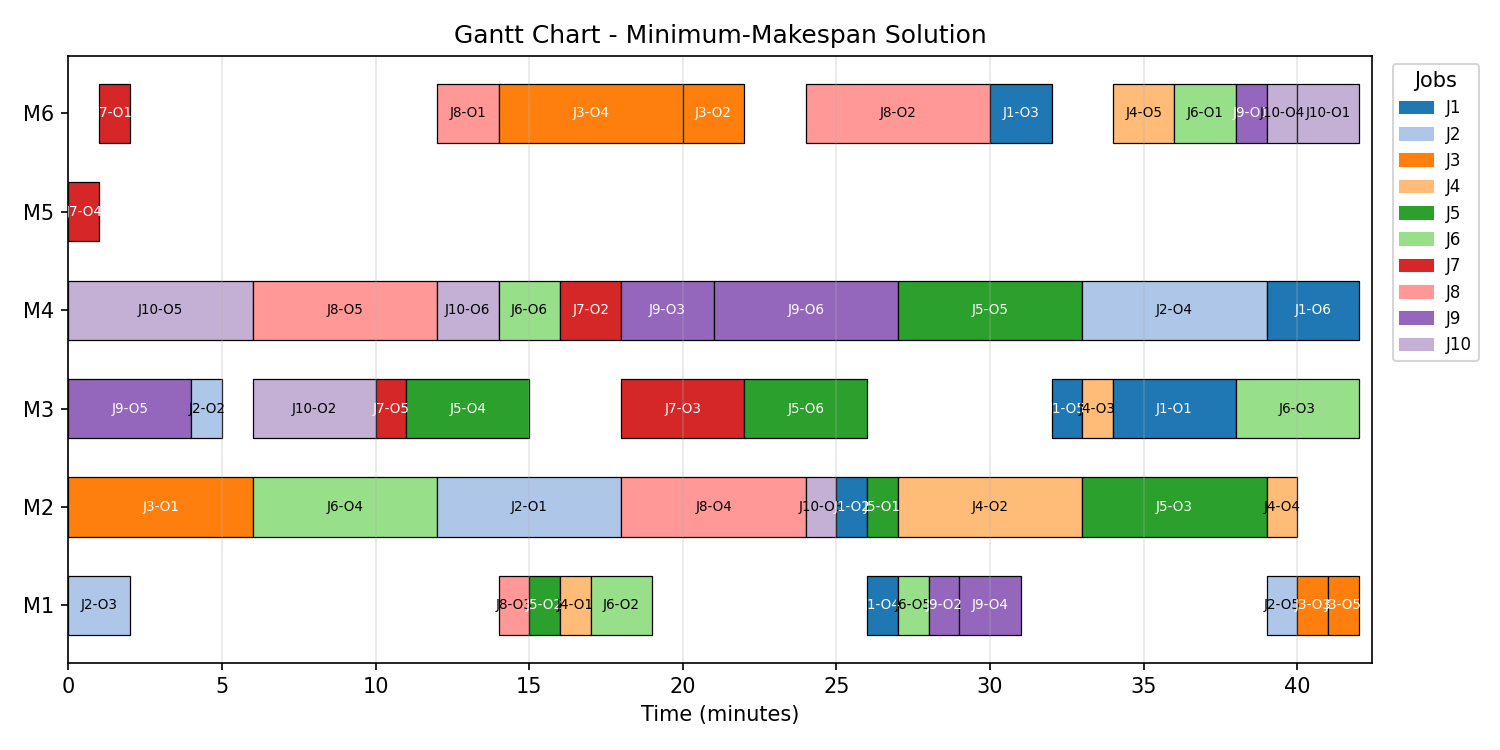
\includegraphics[width=0.95\textwidth]{gantt_chart.png}
    \caption{Gantt chart of the minimum-makespan schedule.}
    \label{fig:gantt-chart}
\end{figure}

% =====================================================================
\section{Discussion: Relationship to Burmeister et al. (2024)}
\label{sec:discussion}
% =====================================================================

This project reproduces the \emph{concept} of a memetic NSGA-II for energy-cost-aware FJSP described
in \citet{burmeister2024memetic}, not their full experimental apparatus. Specifically:

\begin{itemize}
    \item \textbf{Benchmark coverage.} The source paper validates on all fifteen Brandimarte
    instances (mk01--mk15); this project includes and parses ten (mk01--mk10). The remaining five
    (mk11--mk15) are substantially larger and, per the source paper, pushed even an exact Gurobi
    solver to its memory limits; they are out of scope for a mini project run on commodity
    hardware.
    \item \textbf{No exact-solver comparison.} The source paper's central empirical claim is a
    comparison of the memetic NSGA-II's approximated front against an exact Gurobi baseline (with
    epsilon-constraint scalarisation) to quantify solution quality. This project does not implement
    or run that comparison; its Pareto fronts should be read as the algorithm's own output, not as
    validated-optimal.
    \item \textbf{Price series.} The source paper models RTP tariffs at hourly and finer resolution
    over multi-day planning horizons matched to each benchmark instance's scale. This project uses a
    representative one-month hourly Belgian price series, resampled to per-minute resolution.
    \item \textbf{Local search operator.} This project's local search is a simplified greedy
    neighbourhood search over machine reassignment and sequencing swaps; the source paper's operator
    design and parameterisation is more extensive.
    \item \textbf{No rolling horizon.} The source paper discusses extending the method to a
    rolling-horizon setting that reacts to updated price forecasts; this is out of scope here.
\end{itemize}

% =====================================================================
\section{Limitations and Future Work}
\label{sec:limitations}
% =====================================================================

\begin{itemize}
    \item \textbf{Computational cost of local search.} The local-search step re-evaluates a full
    neighbourhood every generation ($O(n_{\text{ops}})$ machine moves + $O(n_{\text{ops}}^2)$
    sequencing swaps per offspring), which limits scalability to the largest benchmark instances
    (mk08--mk10, 20 jobs) without further optimisation.
    \item \textbf{No exact baseline.} Adding an exact or near-exact solver comparison (e.g.\ via a
    MILP solver on smaller instances) would let solution quality be quantified rather than only
    visualised.
    \item \textbf{Static price horizon.} The energy price series is fixed for the duration of a run;
    extending to a rolling-horizon setting that incorporates updated price forecasts, as discussed in
    \citet{burmeister2024memetic}, is a natural next step.
\end{itemize}

% =====================================================================
\section{Conclusion}
\label{sec:conclusion}
% =====================================================================

This project implements a memetic NSGA-II for the energy-cost-aware Flexible Job-Shop Scheduling
Problem, combining real Brandimarte benchmark instances with a real electricity price series to
produce genuine, non-trivial makespan/energy-cost trade-offs rather than results based on synthetic
problem instances or assumed energy rates. The approach and its motivation follow
\citet{burmeister2024memetic}; this document has aimed to be explicit about what is reproduced and
what is simplified, in the interest of academic honesty about the project's scope.

% =====================================================================
\bibliographystyle{plainnat}
\bibliography{references}
% =====================================================================

\end{document}
